% -*- root: ../../../main.tex -*-
\subsection{Leader Election}
\label{Leader Election}
In un dato term, tutte le \textit{operazioni di replicazione} del log sono affidate ad un server che ricopre il ruolo di \textit{leader}. Al fine di accordarsi in maniera safe su un unico leader è necessario applicare un protocollo di elezione robusto.  

	\subsubsection{Candidatura}
	Ogni elezione ha inizio nel momento in cui uno o più server si candidano come aspiranti leader.

	\begin{enumerate}
		\item{\textbf{Stato iniziale:}}	ogni server inizialmente si trova nello stato di follower e vi resta fintantochè riceve nuovi messaggi dall'attuale server leader.
		\item{\textbf{Heartbeat:}} il leader, periodicamente, invia un messaggio detto di \textit{heartbeat}\footnote{come heartbeat vengono utilizzati i messaggi di tipo \textit{AppendEntry} che, nel caso in cui non ci sia effettivamente una entry da appendere, vengono lasciati vuoti.} 
		per comunicare ai suoi follower che è ancora in funzione.
		\item{\textbf{Timeout:}} i server \textbf{follower} mantengono internamente un \textbf{timer randomico} che si resetta ogni volta che viene ricevuto un messaggio dal leader. La durata di questo timer viene chiamata \textit{election timeout}.		
		\item{\textbf{Inizio candidatura:}} allo scadere del timer, il follower considera il leader assente e si propone come leader effettuando un \textbf{cambiamento di stato} da follower a candidate e dando inizio a una \textbf{nuova leader election}.
	\end{enumerate}


Quando una \textit{Leader Election} ha inizio il follower esegue i seguenti passaggi:

\begin{enumerate}
	\item{\emph{Incrementa di uno il proprio term}}
	\item{\emph{Cambia il proprio stato in candidate}}
	\item{\emph{Vota per sè stesso}}
	\item{\emph{Invia in broadcast un messaggio di tipo ``Request Vote'' affinchè gli altri membri del cluster possano votarlo}}
\end{enumerate}
 
A questo punto possono verificarsi i seguenti tre scenari:
\begin{enumerate}
	\item{\textbf{Il candidate vince l'elezione:}} questo accade quando il numero di voti ricevuti dagli altri membri del cluster (compreso il proprio) raggiunge la maggioranza.\\
	A questo punto \textit{cambia il suo stato in \textbf{leader}} e invia un \textbf{heartbeat}, con lo scopo di controllare il cluster evitando che si inneschino nuove candidature.

	\item{\textbf{Un altro candidate vince l'elezione:}} questo può accadere se ad esempio i due si candidano a poca distanza l'uno dall'altro. A questo punto il candidate che ha perso, riceverà un messaggio dal nuovo leader e tornerà follower.
	
	\item{\textbf{Nessuno vince le elezioni:}} la contemporanea presenza di più \textbf{Candidate} può portare a uno \textbf{Split-Vote}, ovvero una situazione in cui nessuno dei candidate ottiene la maggioranza dei voti. In questo caso il \textit{term termina senza aver avuto un leader} e viene dato inizio al term successivo.
\end{enumerate}

  \subsubsection{Elezione: Safety e Liveness}\label{electionsaf}
  Il protocollo di elezione, al fine di essere robusto, deve soddisfare requisiti di safety e di liveness.
  
  \begin{itemize}
    \item{\textbf{No leader multipli }(Election Safety):} non vogliamo che \textbf{più di una macchina} possa essere eletta come leader nel medesimo term.
    \begin{itemize}
      \item{\emph{Proof:}} ogni server rilascia \textbf{un solo voto} per term e lo salva su disco. Se malauguratamente avviene un crash allora, nel caso in cui il server torni operativo, esso verificherà la possibilità di voto recuperando l'informazione dal disco. Quindi possiamo dire che due candidates non possono accumulare due diverse maggioranze sullo stesso term. 
    \end{itemize}
    \item{\textbf{No Elezioni bloccate  }(liveness):} vogliamo evitare che nessun server diventi leader all'infinito.
    \begin{itemize}
      \item{\emph{Proof:}} ogni candidate mantiene internamente un \textbf{timer randomico} che viene inizializzato ad un valore che oscilla tra un massimo e un minimo, come accade per i follower. Questo timer, quando innescato, viene impostato ad un nuovo valore e fa si che il candidate incrementi il suo term e invii nuovamente delle \textit{Request-Vote} a tutto il cluster, come se si fosse ricandidato. Facendo uso di questo espediente si minimizza la possibilità che si verifichino consecutivamente più \textit{Split-Vote}. Questo garantisce che le elezioni possano, prima o poi, progredire portando all'elezione di un leader in un futuro term.\\
      Il meccanismo funziona se il valore di timeout è settato a un valore maggiore del \textbf{RTT} di una comunicazione broadcast. Solitamente il valore scelto si aggira intorno ai 150/300 ms.
      \[
        T > broadcastRTT
      \] 
    \end{itemize} 
  \end{itemize}  

\begin{figure}[H]
	\centering
	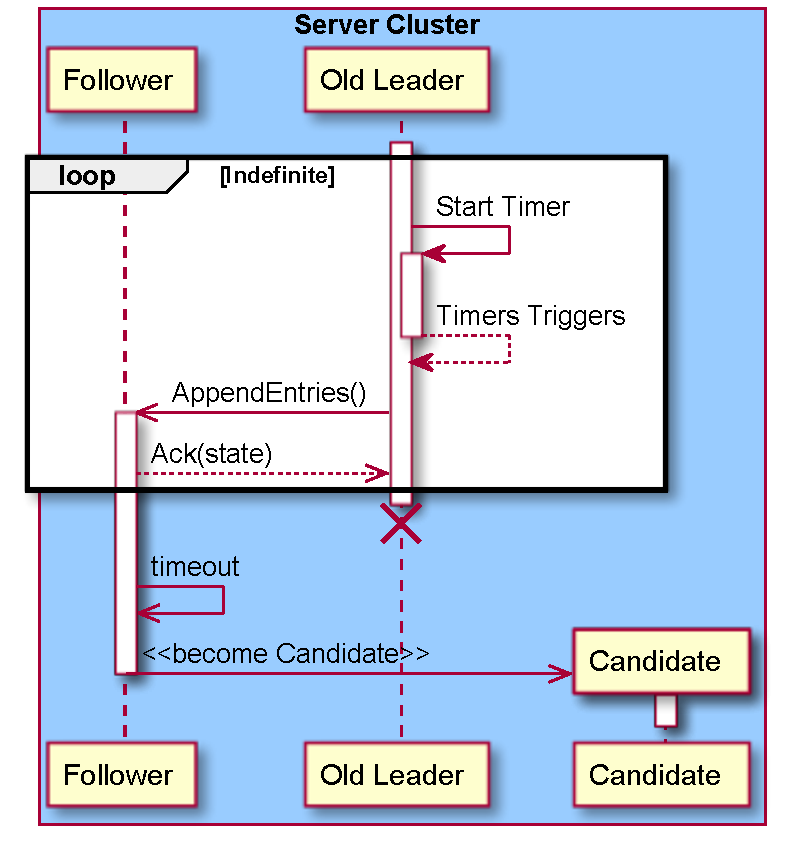
\includegraphics[width=0.70\columnwidth]{seqDiagrams/Candidatura}
  \captionsetup{singlelinecheck=off}
  \caption[stateDiagramCaption]{
  Uno scenario semplificato in cui viene mostrata una \textit{Leader Election}
    \begin{enumerate}
      \setlength\itemsep{0em}
      \item{Il vecchio leader inizialmente svolge correttamente le sue mansioni, divulgando periodicamente i propri \textit{heartbeats}}
      \item{Successivamente il leader subisce un \textbf{fault} e di conseguenza non riesce più a svolgere le proprie attività}
      \item{Prima o poi, non ricevendo più notizie dal leader, uno dei follower vedrà scadere il proprio timer}.
    \end{enumerate}}
	\label{fig:figure4}
\end{figure}

\begin{figure}[H]
  \centering
  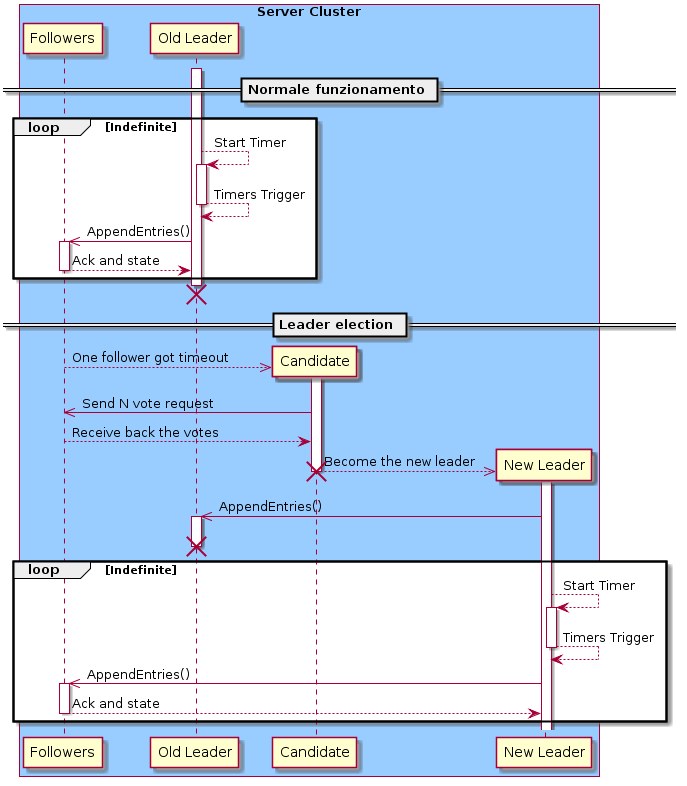
\includegraphics[width=0.99\columnwidth]{seqDiagrams/LeaderElection}
  \captionsetup{singlelinecheck=off}
  \caption[stateDiagramCaption]{
  Uno scenario semplificato in cui viene mostrata una \textit{Leader Election}
    \begin{enumerate}
      \setlength\itemsep{0em}
      \item{Diventato candidate, esso procederà a inviare le \textit{Vote request} a tutti i follower del cluster}.
      \item{Ricevuta la maggioranza dei voti verrà eletto leader e ripristinerà il normale funzionamento del cluster.}
      \item{Il vecchio leader quando tornerà on-line riceverà un \textit{AppendEntry} e tornerà allo stato di follower}.
    \end{enumerate}}
  \label{fig:figure5}
\end{figure}

